\documentclass{standalone}
\usepackage{tikz}
\usetikzlibrary{calc}
\usepackage{amsmath}

\begin{document}

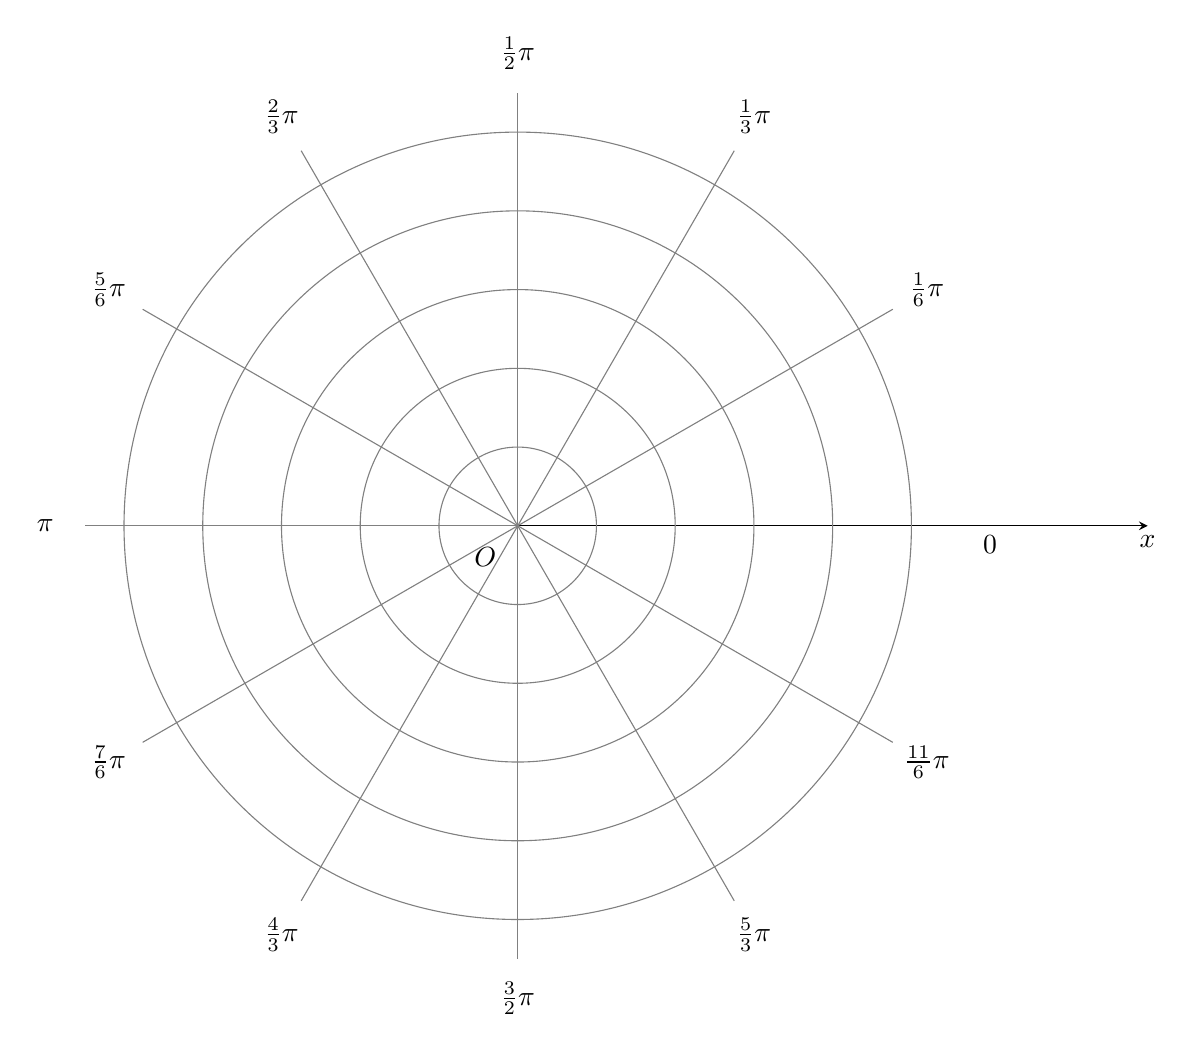
\begin{tikzpicture}
\draw [-stealth] (0,0) -- (8,0) node [below] {$x$};
\node at (0:0) [below left=0.15cm] {$O$};
\node at (0:6) [below] {$0$};
\foreach \deg / \rad in {30/$\frac{1}{6}\pi$, 60/$\frac{1}{3}\pi$, 90/$\frac{1}{2}\pi$, 
	120/$\frac{2}{3}\pi$, 150/$\frac{5}{6}\pi$, 180/$\pi$, 
	210/$\frac{7}{6}\pi$, 240/$\frac{4}{3}\pi$, 270/$\frac{3}{2}\pi$, 
	300/$\frac{5}{3}\pi$, 330/$\frac{11}{6}\pi$} {
	\draw [gray] (0:0) -- (\deg:5.5);
	\node at (\deg:6)  {\rad};
}

\foreach \r in {1,...,5}
	\draw [gray] (0:0) circle(\r);
\end{tikzpicture}

\end{document}